\documentclass{beamer}
\usetheme{Madrid}
\usecolortheme{default}

% Packages
\usepackage{listings}
\usepackage{xcolor}
\usepackage{hyperref}
\usepackage{graphicx}
\usepackage{tikz}
\usepackage{booktabs}
\usepackage{adjustbox}
\usetikzlibrary{shapes.geometric, arrows, positioning, fit, backgrounds}

% Code listing style
\lstset{
    basicstyle=\tiny\ttfamily,
    keywordstyle=\color{blue},
    commentstyle=\color{green!60!black},
    stringstyle=\color{orange},
    breaklines=true,
    frame=single,
    backgroundcolor=\color{gray!10},
    showstringspaces=false
}

% Python style
\lstdefinestyle{python}{
    language=Python,
    morekeywords={self, True, False, None, str, int, bool, list, dict, Optional}
}

% UofT colors
\definecolor{uoftblue}{RGB}{6,41,88}
\setbeamercolor{titlelike}{bg=uoftblue}
\setbeamerfont{title}{series=\bfseries}

\title[Learning Agent]
{Co-Evolving Action and Environment Understanding\\in Unknown Domains}

\subtitle{A Vision-Language Model Approach to ARC-AGI-3}

\author[Your Name]
{Your Name}

\institute[UofT]
{
  University of Toronto\\
  Master's Research
}

\date[December 2024]
{Supervisor Meeting, December 2024}

\begin{document}

% =============================================================================
% TITLE
% =============================================================================
\frame{\titlepage}

% =============================================================================
% TABLE OF CONTENTS
% =============================================================================
\begin{frame}
\frametitle{Table of Contents}
\tableofcontents
\end{frame}

% =============================================================================
\section{The Problem: ARC-3 as Policy Learning}
% =============================================================================

\begin{frame}
\frametitle{ARC-3: The Core Challenge}

\begin{center}
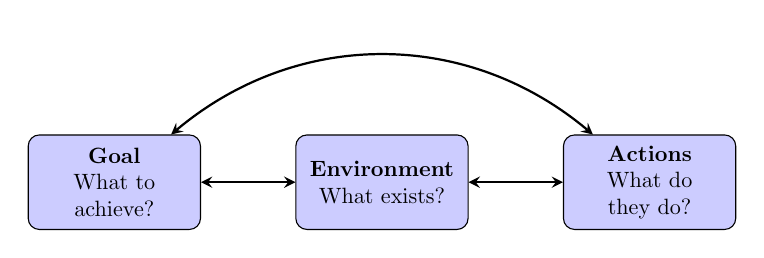
\begin{tikzpicture}[scale=0.8, transform shape]
\tikzstyle{discover} = [rectangle, draw, fill=blue!20, text width=2.5cm, text centered, minimum height=1.5cm, rounded corners]
\tikzstyle{arrow} = [thick, <->, >=stealth]

\node (goal) [discover] {\textbf{Goal}\\What to achieve?};
\node (env) [discover, right=1.5cm of goal] {\textbf{Environment}\\What exists?};
\node (actions) [discover, right=1.5cm of env] {\textbf{Actions}\\What do they do?};

\draw [arrow] (goal) -- (env);
\draw [arrow] (env) -- (actions);
\draw [arrow, bend left=40] (goal) to (actions);

\end{tikzpicture}
\end{center}

\vspace{1em}

\begin{alertblock}{Key Insight}
These \textbf{cannot} be learned in isolation — they must \textbf{co-evolve}.
\end{alertblock}

\end{frame}

% SPEAKER NOTES:
% - This is a chicken-and-egg problem
% - You can't understand "move player left" without knowing what a "player" is
% - You discover what a "player" is by seeing what moves when you press buttons
% - Unlike standard RL, there's no reward signal until you discover the goal
% - ARC Prize 2024: state-of-art improved from 33% to 55.5%
% - But ARC-3 is interactive, not static puzzles - entirely new challenge

% =============================================================================
\begin{frame}
\frametitle{The Chicken-and-Egg Problem}

\begin{center}
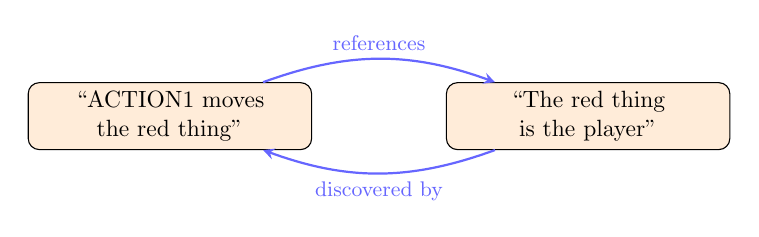
\begin{tikzpicture}[scale=0.85, transform shape]
\tikzstyle{concept} = [rectangle, draw, fill=orange!15, text width=4cm, text centered, minimum height=1cm, rounded corners]
\tikzstyle{arrow} = [thick, ->, >=stealth, blue!60]

\node (action) [concept] {``ACTION1 moves\\the red thing''};
\node (object) [concept, right=2cm of action] {``The red thing\\is the player''};

\draw [arrow, bend left=20] (action) to node[above, font=\small] {references} (object);
\draw [arrow, bend left=20] (object) to node[below, font=\small] {discovered by} (action);

\end{tikzpicture}
\end{center}

\vspace{1.5em}

\textbf{Actions} are defined using \textbf{objects}

\textbf{Objects} are discovered through \textbf{actions}

\vspace{1em}

$\Rightarrow$ Must learn \textit{both simultaneously}

\end{frame}

% SPEAKER NOTES:
% - Actions reference objects: "ACTION1 moves the red thing"
% - Roles inferred from actions: "The red thing is probably the player"
% - This bidirectional dependency is why standard approaches fail
% - Can't learn actions first (don't know objects)
% - Can't learn objects first (don't know what responds to input)

% =============================================================================
\begin{frame}
\frametitle{The Original Vision}

\begin{center}
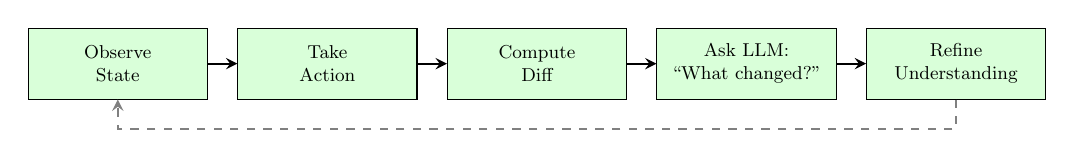
\begin{tikzpicture}[scale=0.75, transform shape]
\tikzstyle{stepbox} = [rectangle, draw, fill=green!15, text width=2.8cm, text centered, minimum height=1.2cm, font=\small]
\tikzstyle{arrow} = [thick, ->, >=stealth]

\node (obs) [stepbox] {Observe\\State};
\node (act) [stepbox, right=0.5cm of obs] {Take\\Action};
\node (diff) [stepbox, right=0.5cm of act] {Compute\\Diff};
\node (ask) [stepbox, right=0.5cm of diff] {Ask LLM:\\``What changed?''};
\node (ref) [stepbox, right=0.5cm of ask] {Refine\\Understanding};

\draw [arrow] (obs) -- (act);
\draw [arrow] (act) -- (diff);
\draw [arrow] (diff) -- (ask);
\draw [arrow] (ask) -- (ref);
\draw [arrow, dashed, gray] (ref.south) -- ++(0,-0.5) -| (obs.south);

\end{tikzpicture}
\end{center}

\vspace{1em}

\begin{block}{First Goal}
Don't solve the game — \textbf{understand the world first}.
\end{block}

\end{frame}

% SPEAKER NOTES:
% - Build understanding before attempting to solve
% - Capture board state, take action, observe change
% - Store before/after as images + compute diff
% - Ask LLM: "What changed? What does this action do?"
% - Iteratively refine until consistent understanding
% - Environment and action understanding develop TOGETHER
% - Terminate after learning - goal discovery comes later

% =============================================================================
\section{Dead Ends: What Didn't Work}
% =============================================================================

\begin{frame}
\frametitle{Dead End \#1: CNN Binary Predictor}

\begin{columns}[T]
\begin{column}{0.45\textwidth}
\textbf{The Idea}
\begin{itemize}
    \item Train CNN at test-time
    \item Predict: will action change frame?
\end{itemize}

\vspace{1em}
\textbf{The Problem}
\begin{itemize}
    \item Output: \texttt{True/False}
    \item Learns \textit{that} something changed
    \item Not \textit{what} or \textit{how}
\end{itemize}
\end{column}

\begin{column}{0.5\textwidth}
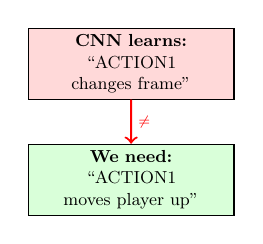
\begin{tikzpicture}[scale=0.7, transform shape]
\tikzstyle{box} = [rectangle, draw, text width=3.5cm, text centered, minimum height=0.8cm, font=\small]

\node (cnn) [box, fill=red!15] {\textbf{CNN learns:}\\``ACTION1 changes frame''};
\node (need) [box, fill=green!15, below=0.8cm of cnn] {\textbf{We need:}\\``ACTION1 moves player up''};

\draw [thick, red, ->] (cnn) -- node[right, font=\scriptsize] {$\neq$} (need);
\end{tikzpicture}
\end{column}
\end{columns}

\vspace{1em}

\begin{alertblock}{Verdict}
Binary signal = zero information for learning mechanics.
\end{alertblock}

\end{frame}

% SPEAKER NOTES:
% - Seemed promising at first: learn which actions are "interesting"
% - THE fundamental flaw: frame_changed = True/False
% - You can learn "ACTION1 usually changes the frame"
% - But you learn NOTHING about WHAT it does
% - Can't build a plan from binary signals
% - A vision-based NN at test-time will never predict outcomes meaningfully
% - Full implementation in agents/templates/action_agent.py

% =============================================================================
\begin{frame}
\frametitle{Dead End \#2: Direct VLM Prompting}

\begin{columns}[T]
\begin{column}{0.48\textwidth}
\textbf{The Idea}
\begin{itemize}
    \item Send raw 64×64 grid to VLM
    \item Ask: ``What action should I take?''
\end{itemize}

\vspace{0.8em}
\textbf{What Happened}
\begin{itemize}
    \item 400K tokens in 6 actions
    \item Wrong position assumptions
    \item No state change detection
    \item Hallucinated game mechanics
\end{itemize}
\end{column}

\begin{column}{0.48\textwidth}
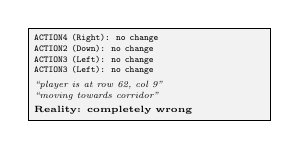
\begin{tikzpicture}[scale=0.65, transform shape]
\tikzstyle{logbox} = [rectangle, draw, fill=gray!10, text width=4.5cm, font=\tiny, align=left]

\node (log) [logbox] {
\texttt{ACTION4 (Right): no change}\\
\texttt{ACTION2 (Down): no change}\\
\texttt{ACTION3 (Left): no change}\\
\texttt{ACTION3 (Left): no change}\\[0.3em]
\textit{``player is at row 62, col 9''}\\
\textit{``moving towards corridor''}\\[0.3em]
\textbf{Reality: completely wrong}
};

\end{tikzpicture}
\end{column}
\end{columns}

\vspace{0.8em}

\begin{alertblock}{Verdict}
VLMs can't track state without structured before/after analysis.
\end{alertblock}

\end{frame}

% SPEAKER NOTES:
% - Tested with Gemini 3.0 Pro via OpenRouter
% - Sent raw 64x64 integer grid as text
% - Model made detailed observations but they were WRONG
% - Example: "player is at row 62, col 9" - completely fabricated
% - No mechanism to verify claims against actual state changes
% - Token cost exploded: ~70K tokens per action (observation + action)
% - After 6 actions: 400K tokens consumed with zero correct understanding
% - The model SOUNDS confident but has no grounding in reality
% - This is why we need structured before/after comparison
% - Full implementation in agents/templates/llm_agents.py (OpenRouterLLM class)

% =============================================================================
\begin{frame}
\frametitle{Dead End \#3: RL-Based Policy Learning}

\begin{center}
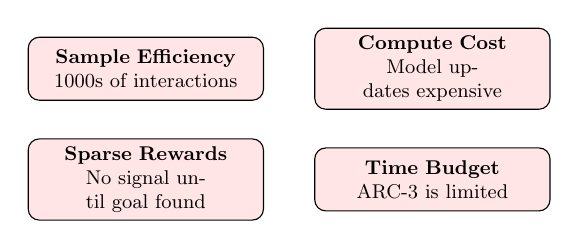
\begin{tikzpicture}[scale=0.8, transform shape]
\tikzstyle{problem} = [rectangle, draw, fill=red!10, text width=3.5cm, text centered, minimum height=1cm, rounded corners, font=\small]

\node (sample) [problem] {\textbf{Sample Efficiency}\\1000s of interactions};
\node (compute) [problem, right=0.8cm of sample] {\textbf{Compute Cost}\\Model updates expensive};
\node (reward) [problem, below=0.6cm of sample] {\textbf{Sparse Rewards}\\No signal until goal found};
\node (time) [problem, below=0.6cm of compute] {\textbf{Time Budget}\\ARC-3 is limited};

\end{tikzpicture}
\end{center}

\vspace{1em}

\begin{alertblock}{Core Problem}
Even sample-efficient RL needs too many interactions for test-time.
\end{alertblock}

\end{frame}

% SPEAKER NOTES:
% - Model-based RL is more sample efficient than model-free
% - But still requires hundreds of interactions minimum
% - Test-time: maybe 10 minutes, few hundred actions
% - No reward signal means no gradient for learning
% - Would need to discover goal before learning anything useful
% - Value Equivalence (Grimm 2020, 2021) helps efficiency but still needs training

% =============================================================================
\begin{frame}
\frametitle{Related Work: The Gap}

\begin{center}
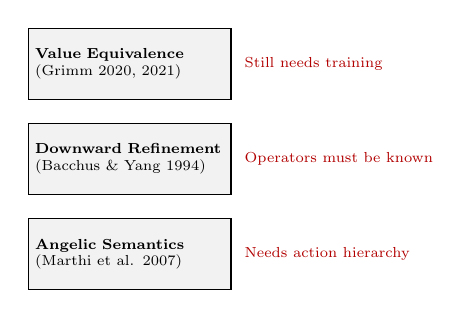
\begin{tikzpicture}[scale=0.75, transform shape]
\tikzstyle{work} = [rectangle, draw, fill=gray!10, text width=3.2cm, minimum height=1.2cm, font=\scriptsize, align=left]
\tikzstyle{limit} = [font=\scriptsize\color{red!70!black}]

\node (ve) [work] {\textbf{Value Equivalence}\\(Grimm 2020, 2021)};
\node (ve_lim) [limit, right=0.1cm of ve] {Still needs training};

\node (dr) [work, below=0.4cm of ve] {\textbf{Downward Refinement}\\(Bacchus \& Yang 1994)};
\node (dr_lim) [limit, right=0.1cm of dr] {Operators must be known};

\node (as) [work, below=0.4cm of dr] {\textbf{Angelic Semantics}\\(Marthi et al. 2007)};
\node (as_lim) [limit, right=0.1cm of as] {Needs action hierarchy};

\end{tikzpicture}
\end{center}

\vspace{0.5em}

\begin{alertblock}{Gap in Literature}
None solve: ``Learn operators from scratch at test-time.''
\end{alertblock}

\end{frame}

% SPEAKER NOTES:
% - Value Equivalence Principle: great for efficient RL modeling, but still needs training
% - Proper Value Equivalence: refined theory, doesn't solve test-time cost
% - Downward Refinement: hierarchical planning, assumes operators are KNOWN
% - Angelic Semantics: optimistic/pessimistic bounds, needs prior action hierarchy
% - Our problem: discover operators from scratch with no prior
% - Connection to spectral methods (Ng et al.): grouping by similarity

% =============================================================================
\section{The Solution: VLM as Reasoning Engine}
% =============================================================================

\begin{frame}
\frametitle{Key Insight: VLM as Reasoning Engine}

\begin{center}
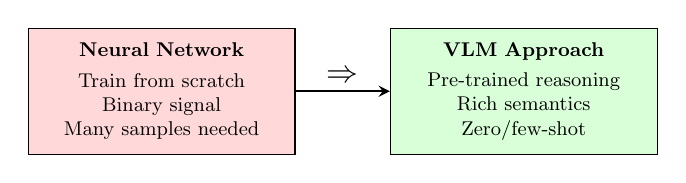
\begin{tikzpicture}[scale=0.8, transform shape]
\tikzstyle{approach} = [rectangle, draw, text width=4cm, text centered, minimum height=2cm, font=\small]

\node (nn) [approach, fill=red!15] {\textbf{Neural Network}\\[0.3em]Train from scratch\\Binary signal\\Many samples needed};
\node (vlm) [approach, fill=green!15, right=1.5cm of nn] {\textbf{VLM Approach}\\[0.3em]Pre-trained reasoning\\Rich semantics\\Zero/few-shot};

\draw [thick, ->, >=stealth] (nn) -- node[above] {\Large $\Rightarrow$} (vlm);

\end{tikzpicture}
\end{center}

\vspace{1em}

\textbf{VLM provides:}
\quad Object recognition \quad|\quad Causal reasoning \quad|\quad Hypothesis testing

\end{frame}

% SPEAKER NOTES:
% - Paradigm shift: from learning TO using pre-trained reasoning
% - VLM has already learned about objects, space, causality
% - We just need to prompt it correctly
% - No backpropagation, no gradient updates during test
% - Trade-off: requires sufficient model capacity
% - This is why model choice matters critically

% =============================================================================
\begin{frame}
\frametitle{The Prior Knowledge Problem}

\begin{center}
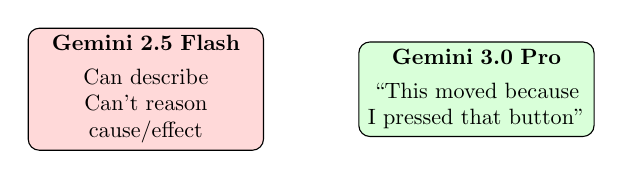
\begin{tikzpicture}[scale=0.8, transform shape]
\tikzstyle{model} = [rectangle, draw, text width=3.5cm, text centered, minimum height=1.5cm, rounded corners]

\node (flash) [model, fill=red!15] {\textbf{Gemini 2.5 Flash}\\[0.3em]Can describe\\Can't reason cause/effect};
\node (pro) [model, fill=green!15, right=1.5cm of flash] {\textbf{Gemini 3.0 Pro}\\[0.3em]``This moved because\\I pressed that button''};

\end{tikzpicture}
\end{center}

\vspace{1em}

\begin{block}{Finding}
The bottleneck isn't game knowledge — it's \textbf{reasoning capacity}.
\end{block}

\vspace{0.5em}
{\small Required: Spatial reasoning, object permanence, cause-effect inference}

\end{frame}

% SPEAKER NOTES:
% - Surprising finding: bottleneck isn't game-specific knowledge
% - Both models have never seen ARC-3
% - Difference is REASONING CAPACITY
% - Gemini 2.5 Flash: can describe what it sees, can't reason about cause/effect
% - Gemini 3.0 Pro: understands "this moved because I pressed that button"
% - Supports VideoGameBench findings: even Gemini 2.5 Pro only completed 0.48% of games
% - Knowledge cutoff January 2025 - safe for evaluation

% =============================================================================
\begin{frame}
\frametitle{The Gestalt Gap in VLMs}

\begin{center}
\begin{tikzpicture}[scale=0.9, transform shape]
% Raw grid
\node (raw) at (0,0) {
\begin{tikzpicture}[scale=0.25]
\draw[fill=black] (0,0) rectangle (6,6);
\draw[fill=red] (2,2) rectangle (4,4);
\draw[fill=gray] (0,0) rectangle (6,0.5);
\draw[fill=gray] (0,5.5) rectangle (6,6);
\end{tikzpicture}
};
\node [below=0.1cm of raw, font=\scriptsize] {64×64 pixel grid};

% Arrow
\node at (2.5,0) {\Large $\rightarrow$};

% VLM sees
\node (vlm) at (4.5,0) [rectangle, draw, fill=red!10, text width=2cm, text centered, font=\small] {VLM sees:\\``numbers''};

% We need
\node at (6.5,0) {\Large $\rightarrow$};
\node (need) at (9,0) [rectangle, draw, fill=green!10, text width=2.5cm, text centered, font=\small] {We need:\\``red square\\at (2,2)''};

\end{tikzpicture}
\end{center}

\vspace{1em}

\textbf{Missing Gestalt principles:}
\begin{itemize}
    \item \textbf{Proximity} — adjacent same-color pixels = one object
    \item \textbf{Similarity} — same color suggests same category
    \item \textbf{Common fate} — pixels that move together are one object
\end{itemize}

\end{frame}

% SPEAKER NOTES:
% - VLMs process images holistically but struggle with pixel grids specifically
% - Object-centric models struggle at representation-manipulation boundary
% - Our solution: explicit preprocessing layer
% - Uses scipy.ndimage for connected components
% - 8-connectivity: diagonal pixels count as connected
% - Open research question: can this be learned end-to-end?

% =============================================================================
\begin{frame}
\frametitle{Solution: Object Detection Layer}

\begin{center}
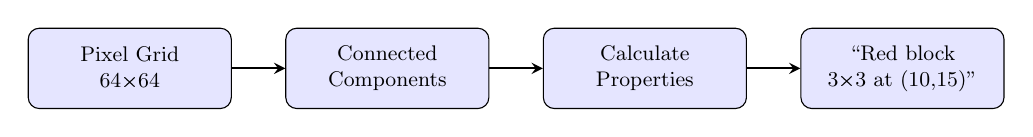
\begin{tikzpicture}[scale=0.85, transform shape]
\tikzstyle{stepbox} = [rectangle, draw, fill=blue!10, text width=2.8cm, text centered, minimum height=1.2cm, font=\small, rounded corners]
\tikzstyle{arrow} = [thick, ->, >=stealth]

\node (pixels) [stepbox] {Pixel Grid\\64×64};
\node (cc) [stepbox, right=0.8cm of pixels] {Connected\\Components};
\node (props) [stepbox, right=0.8cm of cc] {Calculate\\Properties};
\node (out) [stepbox, right=0.8cm of props] {``Red block\\3×3 at (10,15)''};

\draw [arrow] (pixels) -- (cc);
\draw [arrow] (cc) -- (props);
\draw [arrow] (props) -- (out);

\end{tikzpicture}
\end{center}

\vspace{1em}

\textbf{Properties extracted:}
\begin{columns}[T]
\begin{column}{0.5\textwidth}
\begin{itemize}
    \item Bounding box
    \item Center position
    \item Area (pixel count)
\end{itemize}
\end{column}
\begin{column}{0.5\textwidth}
\begin{itemize}
    \item Shape (rectangular?)
    \item Color
    \item Adjacencies
\end{itemize}
\end{column}
\end{columns}

\end{frame}

% SPEAKER NOTES:
% - Uses scipy's ndimage.label for connected components
% - 8-connectivity: diagonal pixels count as connected
% - is_rectangular: does it fill 90%+ of bounding box?
% - Groups pixels into meaningful objects for LLM
% - Output: "Color 2 rectangular block (3x3) at (10,15)"
% - Full implementation in object_detection.py

% =============================================================================
\section{Three-Phase LLM Architecture}
% =============================================================================

\begin{frame}
\frametitle{Three-Phase Architecture: Overview}

\begin{center}
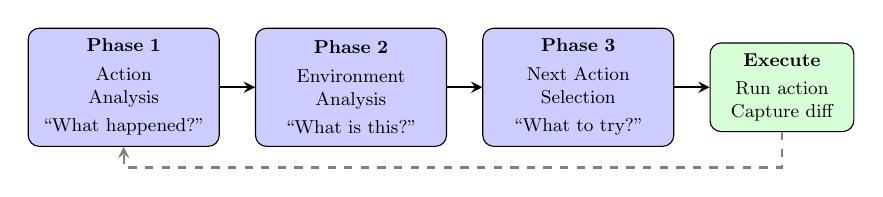
\begin{tikzpicture}[scale=0.75, transform shape]
\tikzstyle{phase} = [rectangle, draw, fill=blue!20, text width=3cm, text centered, minimum height=2cm, rounded corners, font=\small]
\tikzstyle{exec} = [rectangle, draw, fill=green!15, text width=2.2cm, text centered, minimum height=1.5cm, rounded corners, font=\small]
\tikzstyle{arrow} = [thick, ->, >=stealth]

\node (p1) [phase] {\textbf{Phase 1}\\[0.3em]Action\\Analysis\\[0.3em]``What happened?''};
\node (p2) [phase, right=0.6cm of p1] {\textbf{Phase 2}\\[0.3em]Environment\\Analysis\\[0.3em]``What is this?''};
\node (p3) [phase, right=0.6cm of p2] {\textbf{Phase 3}\\[0.3em]Next Action\\Selection\\[0.3em]``What to try?''};
\node (ex) [exec, right=0.6cm of p3] {\textbf{Execute}\\[0.3em]Run action\\Capture diff};

\draw [arrow] (p1) -- (p2);
\draw [arrow] (p2) -- (p3);
\draw [arrow] (p3) -- (ex);
\draw [arrow, dashed, gray] (ex.south) -- ++(0,-0.6) -| (p1.south);

\end{tikzpicture}
\end{center}

\vspace{1em}

\begin{block}{Why Separate?}
Each LLM call has \textbf{one job} with focused context.
\end{block}

\end{frame}

% SPEAKER NOTES:
% - Original vision was single call - didn't work well
% - Separation of concerns: each call has ONE job
% - Benefits: focused context, specialized prompts, independent refinement
% - Environment analysis can self-correct without affecting action analysis
% - Better debugging and logging
% - Full implementation in llm_agents.py

% =============================================================================
\begin{frame}
\frametitle{Phase 1: Action Analysis}

\begin{columns}[T]
\begin{column}{0.45\textwidth}
\textbf{Input}
\begin{itemize}
    \item Before/after images
    \item ASCII grids + diff
    \item Object-level changes
    \item Previous observations
\end{itemize}
\end{column}

\begin{column}{0.45\textwidth}
\textbf{Output}
\begin{itemize}
    \item \texttt{interpretation}
    \item \texttt{had\_effect} (bool)
    \item \texttt{new\_definition}
    \item \texttt{is\_consistent}
\end{itemize}
\end{column}
\end{columns}

\vspace{1em}

\begin{block}{Key Design}
LLM decides whether to \textbf{update} the definition.
\end{block}

{\small\textit{llm\_agents.py:497-700}}

\end{frame}

% SPEAKER NOTES:
% - Most complex prompt, most information provided
% - Images: PNG rendered at 8x scale for visibility
% - ASCII grids provide text fallback for reasoning
% - Object-level diff from Gestalt detector
% - Previous observations for in-context learning
% - update_definition=true only when needed
% - LLM must justify any definition changes

% =============================================================================
\begin{frame}
\frametitle{Phase 2: Environment Analysis}

\begin{columns}[T]
\begin{column}{0.45\textwidth}
\textbf{Discovers}
\begin{itemize}
    \item Background color
    \item Walls and boundaries
    \item Objects and roles
    \item Movement constraints
\end{itemize}
\end{column}

\begin{column}{0.5\textwidth}
\textbf{Role Hypotheses}
\begin{itemize}
    \item ``Red = PLAYER\\(responds to input)''
    \item ``Yellow = COLLECTIBLE\\(disappears on contact)''
\end{itemize}
\end{column}
\end{columns}

\vspace{1em}

\begin{alertblock}{Key Feature}
Can \textbf{correct} previous understanding:\\
``CORRECTION: Red is the player, NOT green.''
\end{alertblock}

{\small\textit{Dedicated LLM call — NOT part of action analysis}}

\end{frame}

% SPEAKER NOTES:
% - Separate call allows independent refinement
% - Role hypotheses are testable predictions
% - Evidence-based: needs justification for claims
% - Can explicitly correct previous mistakes
% - Runs after EVERY action analysis (when state changed)
% - Builds structured EnvironmentKnowledge object
% - Full implementation in llm_agents.py:802-1019

% =============================================================================
\begin{frame}
\frametitle{Phase 3: Next Action Selection}

\textbf{Priority Order:}
\begin{enumerate}
    \item Actions \textbf{never observed} $\rightarrow$ test first
    \item Actions \textbf{needing verification} (< 3 consistent)
    \item Consider: Is current state good for testing?
\end{enumerate}

\vspace{1em}

\begin{block}{Setup Sequences}
\begin{center}
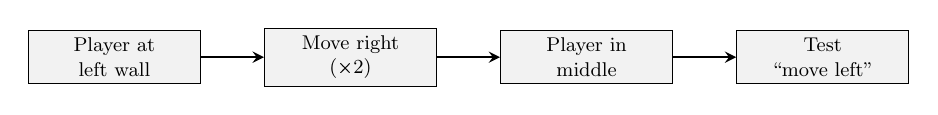
\begin{tikzpicture}[scale=0.8, transform shape]
\tikzstyle{state} = [rectangle, draw, fill=gray!10, text width=2.5cm, text centered, minimum height=0.8cm, font=\small]
\tikzstyle{arrow} = [thick, ->, >=stealth]

\node (bad) [state] {Player at\\left wall};
\node (setup) [state, right=1cm of bad] {Move right\\(×2)};
\node (good) [state, right=1cm of setup] {Player in\\middle};
\node (test) [state, right=1cm of good] {Test\\``move left''};

\draw [arrow] (bad) -- (setup);
\draw [arrow] (setup) -- (good);
\draw [arrow] (good) -- (test);

\end{tikzpicture}
\end{center}
\end{block}

{\small Setup sequences use only \textbf{verified} actions.}

\end{frame}

% SPEAKER NOTES:
% - Not random: strategic exploration
% - Setup sequences critical for avoiding infinite loops
% - Hard guards in agent.py prevent no-op loops
% - If action just had no effect, don't repeat in same state
% - LLM reasons about context suitability
% - Full implementation in llm_agents.py:702-800

% =============================================================================
\begin{frame}[fragile]
\frametitle{Action Analysis Prompt (Key Points)}

\begin{lstlisting}[style=python, basicstyle=\fontsize{5}{6}\selectfont\ttfamily]
ACTION_ANALYSIS_SYSTEM_PROMPT = """You are a game analyst learning how
an unknown game works.

You have NO prior knowledge of this game - base all conclusions on
observed evidence only.

IMPORTANT - CURRENT UNDERSTANDING MAY BE WRONG:
- The environment understanding provided is TENTATIVE
- If what you observe CONTRADICTS the current understanding, note this!

IMPORTANT - UI ELEMENTS AND MOVE COUNTERS:
- There are likely UI elements (dots, squares) that count moves
- Changes in UI elements indicate move consumption, NOT action effects
- Focus on what happened in the PLAY AREA, not just UI changes

Be precise and EVIDENCE-BASED. If you're uncertain, say so."""
\end{lstlisting}

{\small\textit{Full prompt: llm\_agents.py:67-93}}

\end{frame}

% SPEAKER NOTES:
% - Establishes the analyst role
% - NO prior knowledge - pure observation
% - Critical emphasis: current understanding may be WRONG
% - Distinguishes UI changes from game state changes
% - Move counters are common - don't confuse with game effects
% - Evidence-based: don't guess without evidence

% =============================================================================
\begin{frame}[fragile]
\frametitle{Environment Analysis Prompt (Key Points)}

\begin{lstlisting}[style=python, basicstyle=\fontsize{5}{6}\selectfont\ttfamily]
ENVIRONMENT_ANALYSIS_SYSTEM_PROMPT = """You are an environment analyst
studying an unknown game world.

Your SOLE FOCUS is understanding the ENVIRONMENT - not the actions.

CRITICAL: YOUR CURRENT UNDERSTANDING MAY BE WRONG!
- If action results contradict your current understanding, UPDATE IT
- You can and SHOULD replace incorrect objects/roles with better ones

You must discover and document:
1. BOUNDARIES/WALLS - Where can entities NOT move?
2. BACKGROUND - What is the base color/pattern?
3. OBJECTS - What distinct objects exist?
4. OBJECT ROLES - Are some "players"? "Goals"? "Obstacles"?

Be a detective. Make BREAKTHROUGHS. Don't just describe - ANALYZE."""
\end{lstlisting}

{\small\textit{Full prompt: llm\_agents.py:121-160}}

\end{frame}

% SPEAKER NOTES:
% - Sole focus: environment, not actions
% - Critical emphasis: may be WRONG
% - Seven specific things to discover
% - Evidence-based: hypotheses vs confirmed
% - "Be a detective" - active investigation mindset

% =============================================================================
\section{Co-Evolution in Action}
% =============================================================================

\begin{frame}
\frametitle{Co-Evolution: How It Works}

\begin{center}
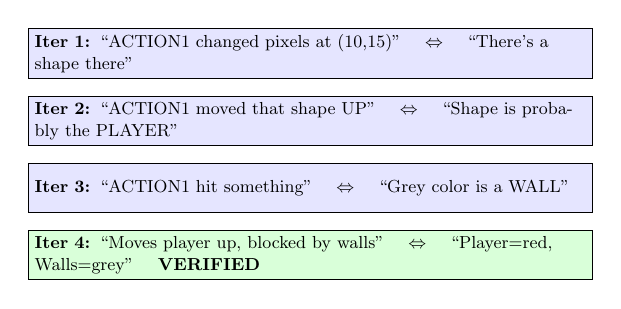
\begin{tikzpicture}[scale=0.7, transform shape]
\tikzstyle{iter} = [rectangle, draw, fill=blue!10, text width=10cm, minimum height=0.9cm, font=\small, align=left]

\node (i1) [iter] {\textbf{Iter 1:} ``ACTION1 changed pixels at (10,15)'' \quad $\Leftrightarrow$ \quad ``There's a shape there''};
\node (i2) [iter, below=0.3cm of i1] {\textbf{Iter 2:} ``ACTION1 moved that shape UP'' \quad $\Leftrightarrow$ \quad ``Shape is probably the PLAYER''};
\node (i3) [iter, below=0.3cm of i2] {\textbf{Iter 3:} ``ACTION1 hit something'' \quad $\Leftrightarrow$ \quad ``Grey color is a WALL''};
\node (i4) [iter, below=0.3cm of i3, fill=green!15] {\textbf{Iter 4:} ``Moves player up, blocked by walls'' \quad $\Leftrightarrow$ \quad ``Player=red, Walls=grey'' \quad \textbf{VERIFIED}};

\end{tikzpicture}
\end{center}

\vspace{1em}

\begin{block}{Bidirectional Building}
Actions defined using objects $\leftrightarrow$ Objects discovered through actions
\end{block}

\end{frame}

% SPEAKER NOTES:
% - Show how each iteration adds to BOTH understandings
% - Iteration 1: raw observation, minimal understanding
% - Iteration 2: object-level thinking, role hypothesis forms
% - Iteration 3: constraint discovery from no-effect
% - Iteration 4: verified understanding, definitions reference each other
% - This is the core innovation: simultaneous learning

% =============================================================================
\begin{frame}
\frametitle{Verification Logic}

\begin{center}
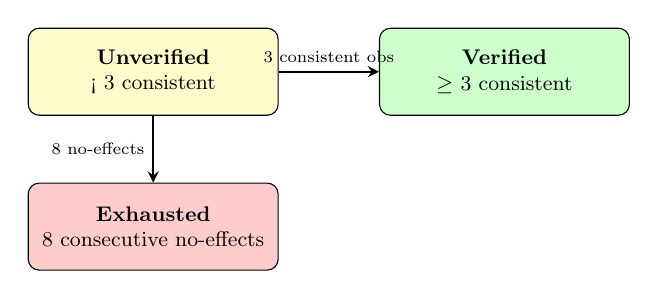
\begin{tikzpicture}[scale=0.85, transform shape]
\tikzstyle{state} = [rectangle, draw, text width=3.5cm, text centered, minimum height=1.3cm, rounded corners, font=\small]

\node (unverified) [state, fill=yellow!20] {\textbf{Unverified}\\< 3 consistent};
\node (verified) [state, fill=green!20, right=1.5cm of unverified] {\textbf{Verified}\\$\geq$ 3 consistent};
\node (exhausted) [state, fill=red!20, below=1cm of unverified] {\textbf{Exhausted}\\8 consecutive no-effects};

\draw [thick, ->, >=stealth] (unverified) -- node[above, font=\scriptsize] {3 consistent obs} (verified);
\draw [thick, ->, >=stealth] (unverified) -- node[left, font=\scriptsize] {8 no-effects} (exhausted);

\end{tikzpicture}
\end{center}

\vspace{1em}

\begin{alertblock}{Key Insight}
Expected no-ops count as ``consistent.''\\
{\small (Hitting the same wall twice = consistent behavior)}
\end{alertblock}

\end{frame}

% SPEAKER NOTES:
% - Every observation counts toward attempts
% - Verified: 3 consecutive consistent observations
% - Exhausted: 8 consecutive no-effects
% - Single effective action resets no-effect counter
% - Expected no-ops: hitting known wall is "consistent"
% - Full logic in models.py, ActionKnowledge class

% =============================================================================
\section{Results}
% =============================================================================

\begin{frame}
\frametitle{Results: It Works!}

\begin{columns}[T]
\begin{column}{0.48\textwidth}
\textbf{Demonstrated}
\begin{itemize}
    \item[$\checkmark$] Discovers action semantics
    \item[$\checkmark$] Builds environment model
    \item[$\checkmark$] Identifies object roles
    \item[$\checkmark$] Handles constraints
    \item[$\checkmark$] Adapts to new stages
\end{itemize}
\end{column}

\begin{column}{0.48\textwidth}
\textbf{Example Outputs}

{\small\textit{Learned definition:}}\\
{\scriptsize ``Moves player UP, blocked by grey walls''}

\vspace{0.5em}
{\small\textit{Breakthrough:}}\\
{\scriptsize ``Grey (5) represents walls — explains all previous no-effects''}
\end{column}
\end{columns}

\vspace{1em}

\begin{block}{Status}
Ready for goal discovery and planning phase.
\end{block}

\end{frame}

% SPEAKER NOTES:
% - All core capabilities demonstrated and working
% - Definitions are semantic, not pixel-level
% - Breakthroughs show genuine insight formation
% - "Grey represents walls" - explains past no-effects retroactively
% - Be prepared to show actual logged output if asked
% - Ready for goal discovery phase

% =============================================================================
\begin{frame}
\frametitle{Comparison with Related Work}

\begin{center}
\begin{tabular}{lccc}
\toprule
\textbf{Approach} & \textbf{Test-Time} & \textbf{From Scratch} & \textbf{Semantic} \\
\midrule
Value Equiv. RL & \textcolor{red}{$\times$} & Via reward & \textcolor{red}{$\times$} \\
Hierarchical Planning & \textcolor{green}{$\checkmark$} & \textcolor{red}{$\times$} Known & Partial \\
CNN Binary & \textcolor{green}{$\checkmark$} & \textcolor{red}{$\times$} Binary only & \textcolor{red}{$\times$} \\
\textbf{Our Approach} & \textcolor{green}{$\checkmark$} & \textcolor{green}{$\checkmark$} & \textcolor{green}{$\checkmark$} \\
\bottomrule
\end{tabular}
\end{center}

\vspace{1em}

\begin{alertblock}{Unique Position}
Semantic, interpretable understanding built at test-time from scratch.
\end{alertblock}

\end{frame}

% SPEAKER NOTES:
% - Table shows unique position in literature
% - Only approach with all three properties
% - Spectral clustering connection: grouping by similarity
% - We group by color adjacency (discovered, not predefined)
% - Semantic output enables goal reasoning later

% =============================================================================
\section{Future Work \& Open Questions}
% =============================================================================

\begin{frame}
\frametitle{Current Scope \& Next Steps}

\begin{center}
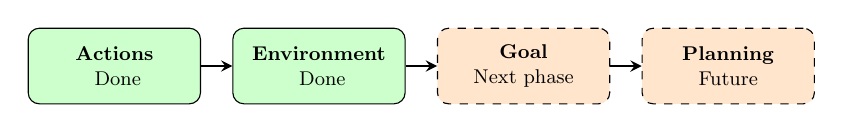
\begin{tikzpicture}[scale=0.8, transform shape]
\tikzstyle{done} = [rectangle, draw, fill=green!20, text width=2.5cm, text centered, minimum height=1.2cm, rounded corners, font=\small]
\tikzstyle{todo} = [rectangle, draw, fill=orange!20, text width=2.5cm, text centered, minimum height=1.2cm, rounded corners, font=\small, dashed]
\tikzstyle{arrow} = [thick, ->, >=stealth]

\node (actions) [done] {\textbf{Actions}\\$\checkmark$ Done};
\node (env) [done, right=0.5cm of actions] {\textbf{Environment}\\$\checkmark$ Done};
\node (goal) [todo, right=0.5cm of env] {\textbf{Goal}\\Next phase};
\node (plan) [todo, right=0.5cm of goal] {\textbf{Planning}\\Future};

\draw [arrow] (actions) -- (env);
\draw [arrow] (env) -- (goal);
\draw [arrow] (goal) -- (plan);

\end{tikzpicture}
\end{center}

\vspace{1em}

\textbf{Foundation complete:}
\begin{itemize}
    \item We know what actions do
    \item We know what objects exist and their roles
    \item We know the constraints
\end{itemize}

$\Rightarrow$ Ready to reason about \textit{what to achieve}

\end{frame}

% SPEAKER NOTES:
% - Scope was intentionally limited to action/env learning
% - Foundation is solid: semantic understanding complete
% - Goal discovery: likely from object roles
% - Planning: use verified definitions as operators
% - Solution generation: execute plan, submit answer
% - Goal discovery not yet implemented - next phase

% =============================================================================
\begin{frame}
\frametitle{Open Research Questions}

\textbf{Q1: End-to-end object detection?}
\begin{itemize}
    \item Current: hand-coded Gestalt grouping
    \item Can VLMs learn this for pixel grids?
\end{itemize}

\vspace{0.5em}

\textbf{Q2: Minimum reasoning capacity?}
\begin{itemize}
    \item 2.5 Flash: insufficient \quad|\quad 3.0 Pro: sufficient
    \item Where is the threshold?
\end{itemize}

\vspace{0.5em}

\textbf{Q3: Cost optimization?}
\begin{itemize}
    \item Currently 3 LLM calls per action
    \item Can we reduce without losing co-evolution?
\end{itemize}

\end{frame}

% SPEAKER NOTES:
% - Q1: Object-centric models struggle at this boundary
% - Could fine-tuning help? Domain-specific training?
% - Q2: Systematic ablation needed
% - What specific reasoning is missing in 2.5 Flash?
% - Q3: Cost optimization for real deployment
% - 3 LLM calls per action is expensive (~$1-5 per game)
% - Could we batch? Reduce frequency of env analysis?

% =============================================================================
\section{Summary}
% =============================================================================

\begin{frame}
\frametitle{Key Takeaways}

\begin{enumerate}
    \item \textbf{Co-evolution is essential}
    \vspace{0.3em}

    \item \textbf{Binary signals don't work} — CNN approach fails
    \vspace{0.3em}

    \item \textbf{RL is too expensive} for test-time learning
    \vspace{0.3em}

    \item \textbf{VLMs provide} pre-trained reasoning\\
    {\small (Requires 3.0 Pro level capacity)}
    \vspace{0.3em}

    \item \textbf{Gestalt gap} needs explicit object detection
    \vspace{0.3em}

    \item \textbf{This approach works} — ready for next phase
\end{enumerate}

\end{frame}

% SPEAKER NOTES:
% - Six key points to remember
% - Co-evolution: the core insight
% - Binary signals: why CNN failed
% - RL: why neural policy learning failed at test-time
% - VLMs: why this works
% - Gestalt: the preprocessing layer needed
% - Works: ready for goal discovery and planning phase

% =============================================================================
\begin{frame}
\frametitle{Architecture Summary}

\begin{center}
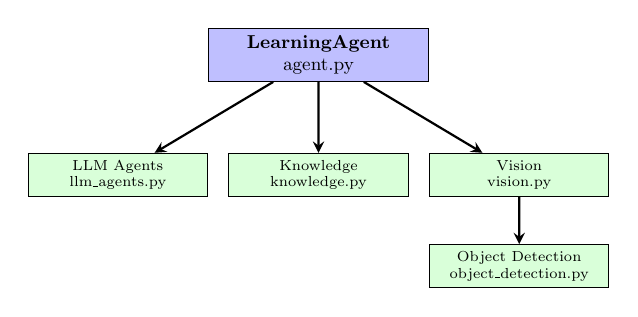
\begin{tikzpicture}[scale=0.75, transform shape]
\tikzstyle{main} = [rectangle, draw, fill=blue!25, text width=3.5cm, text centered, minimum height=0.7cm, font=\small]
\tikzstyle{sub} = [rectangle, draw, fill=green!15, text width=2.8cm, text centered, minimum height=0.6cm, font=\scriptsize]
\tikzstyle{arrow} = [thick, ->, >=stealth]

\node (agent) [main] {\textbf{LearningAgent}\\agent.py};

\node (llm) [sub, below left=1.2cm and 0cm of agent] {LLM Agents\\llm\_agents.py};
\node (know) [sub, below=1.2cm of agent] {Knowledge\\knowledge.py};
\node (vis) [sub, below right=1.2cm and 0cm of agent] {Vision\\vision.py};

\node (obj) [sub, below=0.8cm of vis] {Object Detection\\object\_detection.py};

\draw [arrow] (agent) -- (llm);
\draw [arrow] (agent) -- (know);
\draw [arrow] (agent) -- (vis);
\draw [arrow] (vis) -- (obj);

\end{tikzpicture}
\end{center}

\vspace{0.5em}
{\small\textit{All files in: agents/templates/learning\_agent/}}

\end{frame}

% SPEAKER NOTES:
% - Main orchestration in agent.py
% - Three main components: LLM, Knowledge, Vision
% - Object detection under vision pipeline
% - All models in models.py (Pydantic for serialization)
% - Full implementation ~2000 lines of code
% - Clean separation of concerns

% =============================================================================
\begin{frame}
\frametitle{Questions?}

\begin{center}
\textbf{Key Files}

\vspace{1em}
\begin{tabular}{ll}
\texttt{agent.py} & Main loop \\
\texttt{llm\_agents.py} & Three LLM calls \\
\texttt{knowledge.py} & State management \\
\texttt{models.py} & Data structures \\
\texttt{object\_detection.py} & Gestalt grouping \\
\end{tabular}

\vspace{2em}
\texttt{agents/templates/learning\_agent/}
\end{center}

\end{frame}

% =============================================================================
% REFERENCES
% =============================================================================

\begin{frame}[allowframebreaks]
\frametitle{References}

\begin{thebibliography}{99}

\bibitem{grimm2020value}
Grimm, C., et al. (2020).
\textit{The Value Equivalence Principle for Model-Based RL}.
arXiv:2011.03506.

\bibitem{grimm2021proper}
Grimm, C., et al. (2021).
\textit{Proper Value Equivalence}.
arXiv:2106.10316.

\bibitem{bacchus1994downward}
Bacchus, F., \& Yang, Q. (1994).
\textit{Downward Refinement and Hierarchical Problem Solving}.
AI Journal.

\bibitem{marthi2007angelic}
Marthi, B., et al. (2007).
\textit{Angelic Semantics for High-Level Actions}.
ICAPS.

\bibitem{ng2001spectral}
Ng, A. Y., et al. (2001).
\textit{On Spectral Clustering}.
NeurIPS.

\bibitem{arcprize2024}
ARC Prize. (2024).
\textit{ARC Prize 2024: Technical Report}.
arXiv:2412.04604.

\bibitem{videogamebench}
OpenCV. (2024).
\textit{VideoGameBench}.

\end{thebibliography}

\end{frame}

\end{document}
